\documentclass[11pt]{article}
\usepackage{fullpage}
\usepackage{listings}
\usepackage{needspace}
\usepackage{color}
\usepackage{ifthen}
\usepackage{pgf}
\usepackage{tikz}
\usetikzlibrary{arrows,automata,shapes}
\usepackage{amsmath}
\usepackage{url}
\usepackage{framed}
\usepackage{csc}
\usepackage{textcomp}
\usepackage{multicol}
\usepackage{mathtools}
\DeclarePairedDelimiter\floor{\lfloor}{\rfloor}

\lstset{ %
basicstyle=\footnotesize\ttfamily,       % the size of the fonts that are used for the code
numbers=left,                   % where to put the line-numbers
stepnumber=1,                   % the step between two line-numbers. If it's 1 each line will be numbered
numbersep=5pt,                  % how far the line-numbers are from the code
showspaces=false,               % show spaces adding particular underscores
showstringspaces=false,         % underline spaces within strings
tabsize=4,		                % sets default tabsize to 4 spaces
language=Python,
upquote=true,
columns=fixed
}

\ifthenelse{\isundefined{\isAnswerKey}}
{
    \newenvironment{answer}{\large\lstset{basicstyle=\tiny\ttfamily}\color{white}}{}
}
{
    \newenvironment{answer}{\large\lstset{basicstyle=\large\ttfamily}\color{red}}{}
}

\author{Computer Science Community}
\title{CS-141 Final Exam Review}
\date{\today}

\makeatletter
\let\thetitle\@title
\let\theauthor\@author
\let\thedate\@date
\makeatother

\begin{document}
\header

\begin{enumerate}

\section*{Python Basics}
	\item Python syntax\\
\emph{While most in the CS field will give a fair amount of leeway when it comes to coding by hand,
you nevertheless must have a reasonable level of familiarity with the language's syntax.}

\begin{enumerate}
\item Identify and fix the line(s) that have invalid syntax in the following code:\\
\emph{If the fix for a certain line isn't clear, an explanation of why the line is wrong is sufficient. For this question, assume that one line being incorrect doesn't affect the validity of other lines which may depend on it, where applicable.}
\begin{lstlisting}
include math

int a = 0
b = 0;
c = (int)(0)

for x in range(0, 100):
	print x

def function(int arg):
	return (arg + 2)

sum = b + math.sqrt(c)
total = a + (b ** 0.5)

myList = [1, 2, 3, 4, 5]
for element in myList:
	print(element)

for p in range(0, myList.len()-1):
	print(myList[p])
\end{lstlisting}
\begin{answer}
1 - The idea here is correct, but the line should read "import math", or, alternatively, "from math import *"\\
3 - Python is a dynamically-typed language (as discussed in an earlier question.) You cannot specify a variable's type in this manner.\\
8 - This is valid in syntax in Python 2.x. In Python 3.x, 'print' is a function rather than a statement, thus you need parenthesis to specify arguments to the \texttt{print} function.\\
10 - Like line 3, you cannot specify that a function argument is of a certain type, just that the function argument has a name associated with it. Bonus: How might you go about ensuring that the variable passed in is of the data type you want it to be? (hint - it has something to do with one of the keywords in the list below.)
20 - Close, but no cigar. You want to use the built-in Python statement \texttt{len()} like this: "\texttt{for p in range(0, len(myList)-1):}".
\end{answer}
\\
\item Which of the following are keywords or statements in Python?\\
\texttt{import\hspace{10mm}in\hspace{10mm}from\hspace{10mm}class\hspace{10mm}define\hspace{10mm}int\hspace{10mm}str\hspace{10mm}String}\\
\texttt{True\hspace{9mm}false\hspace{9mm}where\hspace{9mm}while\hspace{9mm}or\hspace{9mm}not\hspace{9mm}isinstance\hspace{9mm}new}\\
\texttt{print\hspace{13mm}range\hspace{13mm}float\hspace{13mm}char\hspace{13mm}bool\hspace{13mm}xor\hspace{13mm}sum}\\
\\
\begin{answer}
All of them except: (\texttt{define, String, false, where, new, xor, char})
\end{answer}
\end{enumerate}





\section*{General Recursion}
	\item %
% NOTE: This question is meant to take up one full page
%	and includes all necessary spacing.
%


Sally is being plagued by an army of lookalike suiters, each of which presents her with an enticing but unbearable meal upon arrival.
The dishes all smell amazing, however, so she can't help but try each one.
A dish will never fail to disappoint her, but fortunately, some of the suiters shared recipes and created identical concoctions.
Once Sally tastes a meal once, she can immediately smell out instances of the same dish and send their bearers away.
\begin{enumerate}
\item
\label{listdupes}
Write a Python function that, given a list of ``dishes,'' returns a list of the rejected dishes in the order they failed to fool her. (e.g. $[1, 2, 2, 3, 3, 3]$ would return [2,3,3] )
\begin{answer}
\begin{lstlisting}
def find_dupes(lst):
	result=[]
	seen=[]
	for member in lst:
		if member not in seen:
			seen.append(member)
		else:
			result.append(member)
	return result
\end{lstlisting}
\end{answer}

\item
If your solution to \ref{listdupes} was iterative, write it recursively; if it was recursive, write it iteratively.
\begin{answer}
\begin{lstlisting}
def find_recur(lst, seen=[]):
	if len(lst)==0:
		return []
	if lst[0] not in seen:
		seen.append(lst[0])
		return find_recur(lst[1:], seen)
	return [lst[0]]+find_recur(lst[1:], seen)
\end{lstlisting}
\textit{or}
\begin{lstlisting}
def find_tail(lst, result=[], seen=[]):
	if len(lst)==0:
		return result
	if lst[0] not in seen:
		seen.append(lst[0])
	else:
		result.append(lst[0])
	return find_tail(lst[1:], result, seen)
\end{lstlisting}
\end{answer}

\item
What is the time complexity of your approach?
Why? \\

\begin{answer}
$O(N^2)$, since the \texttt{seen} list must be searched linearly
\end{answer}
\end{enumerate}

\newpage
	\item \label{reverse()} Write a recursive function that reverses a string (e.g. ``Don't
        get sick'' yields ``kcis teg t'noD'').

\begin{answer}
\begin{lstlisting}
def reverse( string ):
    if string == '' :
        return string
    else:
        return reverse( string[1:] ) + string[0]
\end{lstlisting}
Other solutions are possible.
\end{answer}

	\item Perform a substitution trace on \texttt{reverse('Doge')}.
%\needspace{15\baselineskip}

\begin{answer}
\begin{lstlisting}[numbers=none]
reverse('Doge')
reverse('oge') + 'D'
reverse('ge') + 'o' + 'D'
reverse('e') + 'g' + 'o' + 'D'
'e' + 'g' + 'o' + 'D'
'egoD'
\end{lstlisting}
\end{answer}

\vspace{.5in}
\section*{Files/IO}
	\item Write a function that takes in a file name, and returns the average size of a word in that file. Assume the files will only have 1 word per line, for example:

        \begin{center}
        No\\
        soup\\
        for\\
        you!
        \end{center}

        which has an average length of: 3.25 \\ \emph{Assume a function \texttt{len( str )} which returns the length of a string is provided.}


\begin{answer}
\begin{lstlisting}
def average_wordlength(filename):
    characters = 0
    words = 0
    for line in open(filename):
        words += 1
        characters += len(line)
    return characters/words
\end{lstlisting}
\end{answer}


\newpage
\section*{Tail Recursion}
	\item %
% NOTE: This question is meant to take up one full page
%	and includes all necessary spacing.
%


Below is a function that, given a lower bound \textit{i}, upper bound \textit{n}, and function from integers to integers \textit{f}, computes $\sum\limits_{k=i}^n f(k)$.
\begin{lstlisting}
	def series_sum(i, n, f):
		if(i == n):
			return f(n)
		return f(i) + series_sum(i + 1, n, f)
\end{lstlisting}
\begin{enumerate}
\item Invoke the function to compute $\sum\limits_{k=1}^5 k^2$.
\begin{answer}
\begin{multicols}{3}
\begin{verbatim}
	series_sum(1, 5, lambda x: x**2)
\end{verbatim}
\columnbreak
\hspace{80pt} OR
\columnbreak
\begin{verbatim}
	def square(x): return x**2
	series_sum(1, 5, square)
\end{verbatim}
\end{multicols}
\end{answer}

\item Rewrite the \texttt{series\_sum} function to be tail recursive.
\begin{answer}
\begin{lstlisting}
	def series_sum(i, n, f, s=0):
		if(i == n):
			return s + f(n)
		return series_sum(i + 1, n, f, s + f(i))
\end{lstlisting}
\end{answer}

\vspace{48pt}
\item What is the advantage of the new implementation? \\
\begin{answer}
Tail recursive functions make no additional calculations after the execution of the recursive call completes; thus, they do not necessitate the preservation of stack frames belonging to intermediate recursive invocations.
Provided the language implementation supports sufficient optimization (Note: Python does not), there is no more runtime memory overhead for calling a tail recursive function that makes 100 recursive calls as compared to one that makes none at all.
The true benefit becomes apparent when the recursion depth becomes much deeper: a tail recursive function can handle a recursion depth in the millions, which would cause a non--tail recursive one to overflow the stack.
\end{answer}
\end{enumerate}


\section*{Greedy Algorithms}
	\item Given that an algorithm is \textit{greedy}, is it guaranteed to return an \textit{optimal} solution?

\begin{answer}
NO. Greedy algorithms always choose the \textit{current} best solution,
which is not necessarily the \textit{overall} best solution!
\end{answer}


\newpage
\section*{Structures}
	\item For the sake of this question, you find yourself to be the head programmer under Kim Jong Un's glorious reign.
It also just so happens that a nation-wide track meet is being held today. Thus, the glorious leader has demanded that
you write a program to keep track of information relating to all track runners present at the event.

\begin{enumerate}
\item Write a class named \texttt{TrackRunner} to keep track of all runners competing.
You will need to store their \texttt{name}, \texttt{age}, and \texttt{fastestTime}.
\begin{answer}
\begin{lstlisting}
class TrackRunner:
    __slots__=('name','age','fastestTime')

\end{lstlisting}
\end{answer}

\item Now write a function to make an individual \texttt{TrackRunner} object.
\begin{answer}
\begin{lstlisting}
def makeRunner(r_name,r_age,r_fastestTime):
    runner = TrackRunner()
    runner.name = r_name
    runner.age = r_age
    runner.fastestTime = r_fastestTime
    return runner
\end{lstlisting}
\end{answer}

\item The glorious leader has decided that, on this day, no runner named \texttt{Joe} may win
gold. Given a list of \texttt{TrackRunner} objects, write the function \texttt{aWinnerIsYou(r)} that finds the runner in the list \texttt{r} with the fastest time who's name is not "Joe". 
Then print the runner's name, age and time.
\begin{lstlisting}

\end{lstlisting}
\begin{answer}
\begin{lstlisting}
def aWinnerIsYou(r):
    best = None
    for i in range(len(r)):
        if r[i].name != 'Joe':
            if best == None:
                best = r[i]
            elif best.fastestTime > r[i].fastestTime:
                best = r[i]
    return best

best = aWinnerIsYou(runnersLst)
print(best.name, best.age, best.fastestTime)
\end{lstlisting}
\end{answer}
\end{enumerate}


\newpage
\section*{Stacks and Queues}
	\item How can you use a stack to check if an input string
of exclusively parentheses, brackets, and braces is properly balanced?
(e.g. ``[\{\}]'' is accepted, but ``(()'' and ``[(])'' are not.)\\
Assume that you are provided with a \texttt{Stack} class that has \texttt{push()}, \texttt{pop()}, and \texttt{peek()} member functions.

\begin{answer}
\begin{lstlisting}
def closing_match(char):
	if char == '(':
		return ')'
	elif char == '[':
		return ']'
	elif char == '{':
		return '}'
	elif char == '<':
		return '>'
	else:
		return None

def delims_are_balanced(inString):
    ''' String -> boolean
    Determines if the input string has balanced delimiters.
    Delimiters are () [] {} and <>.
    
    '''
    stack = Stack()
    for char in inString:
        if closing_match(char) != None: # a starting grouping symbol
            stack.push(char)
		else:
			if stack.is_empty():
				return False
			elif char == closing_match(stack.peek()):
				stack.pop()
			else: # mismatched grouping symbol
				return False
    return stack.is_empty()
\end{lstlisting}
\end{answer}

\newpage
\section*{Searching}
	\item Given the sorted list [1, 4, 9, 16, 25, 69, 420, 1337], write out the steps that a binary search would take to find the number 69.
\begin{answer}
\begin{lstlisting}[numbers=none]
[1,4,9,16,|25|,69,420,1337]
[1,4,9,16,25,69,|420|,1337]
[1,4,9,16,25,|69|,420,1337]
\end{lstlisting}
\end{answer}

\vspace{1in}
\section*{Trees}
	\item \begin{enumerate}
	\item If we have a \textbf{balanced} binary search tree containing $n$ nodes:
		\begin{enumerate}
		    \item What is its height? \\
			\begin{answer}
				$\log_2(n)$
			\end{answer}
		    \item How much time would it take to traverse to any of the leaf nodes of this tree? \\
			\begin{answer}
				$\log_2(n)$
			\end{answer}
		    \item What's the worst case search time for an unbalanced search tree? \\
			\begin{answer}
				$n$
			\end{answer}
		\end{enumerate}
	\item How many leaves are in a \textbf{complete} BST containing $n$ nodes? \\
		\begin{answer}
			$\floor*{(n+1)/2}$
		\end{answer}
	\item In terms of runtime efficiency, what is the worst possible configuration (e.g. arrangement of nodes and their children) of a binary search tree? Sketch a small example of what such a configuration looks like. \\
		\begin{answer}
			A perfectly \textit{imbalanced} tree, in which all nodes have one or 0 children. \\

				\begin{tikzpicture}
					\node [draw,ellipse] at (5, 0) (head) {1};
					\node [draw,ellipse] at (7, -.5) (2) {2};
					\node [draw,ellipse] at (9, -1) (3) {3};
					\node [draw,ellipse] at (11, -1.5) (4) {4};
					\node [draw,ellipse] at (13, -2) (5) {5};
					
					\path [draw] (head) -- (2);
					\path [draw] (2) -- (3);
					\path [draw] (3) -- (4);
					\path [draw] (4) -- (5);
				\end{tikzpicture}
			
			
		\end{answer}
	\item Based on your answer above, what data structure is such a BST reminiscent of? \\
		\begin{answer}
			A perfectly imbalanced tree as described above operates like a \textbf{linked list}.
		\end{answer}
\end{enumerate}


\newpage
	\item Write a binary tree class and a function that determines whether one contains a given element.
		\begin{answer}
		\begin{lstlisting}
	class Tree:
		__slots__ = ('head', 'size')

	class TreeNode:
		__slots__ = ('data', 'left', 'right')

	def mkTree(head, size):
		tree = Tree()
		tree.head = head
		tree.size = size
		return tree

	def mkTreeNode(data, left, right):
		tree = Tree()
		tree.data = data
		tree.left = left
		tree.right = right
		return tree

	def is_in_tree(head, element):
		 if head == None:
			return False
		elif head.data == element:
			return True
		elif head.data < element:
			return is_in_tree(head.right, element)
		elif head.data > element:
			return is_in_tree(head.left, element)

	newTree = mkTree(3, mkTreeNode(3, mkTreeNode(1, None, None),
			mkTreeNode(4, None, None)))
	print(is_in_tree(newTree.head, 1)) # -> True
	print(is_in_tree(newTree.head, 3)) # -> True
	print(is_in_tree(newTree.head, 4)) # -> True
	print(is_in_tree(newTree.head, 5)) # -> False
		\end{lstlisting}
		\end{answer}

\newpage
\section*{Heaps}
	\item For a binary heap containing $n$ elements, what is the maximum number of
      swaps occurring after an insert operation?

    \begin{answer}
        log$_{\textrm{2}}$ (n + 1), rounded down.
    \end{answer}

	\item Given a node in an array-based binary heap at index $i$, where are the
      indices of both its children? What is the index of its parent?

    \begin{answer}
    The children are at $2i+1$ and $2i+2$. The parent is at
    $\lfloor\frac{i-1}{2}\rfloor$.

    \marginpar{\small\em Note that in a 1 indexed array system, the children
    would be at $2i$ and $2i+1$. The parent would be at
    $\lfloor\frac{i}{2}\rfloor$.}
    \end{answer}

	\item Run a heap sort in reverse order on the following list: [3,5,1,3,2,7,9], showing the heap
      at each stage. Be sure to heapify the list first.

    \begin{answer}
        Heapify:  \newline
        	[\underline{3}, 5, 1, 3, 2, 7, 9] \newline
    		[\underline{3}, \underline{5}, 1, 3, 2, 7, 9] \newline
    		[\underline{1}, \underline{5}, \underline{3}, 3, 2, 7, 9] \newline
    		[\underline{1}, \underline{3}, \underline{3}, \underline{5}, 2, 7, 9] \newline
    		[\underline{1}, \underline{2}, \underline{3}, \underline{5}, \underline{3}, 7, 9] \newline
    		[\underline{1}, \underline{2}, \underline{3}, \underline{5}, \underline{3}, \underline{7}, 9] \newline
    		[\underline{1}, \underline{2}, \underline{3}, \underline{5}, \underline{3}, \underline{7}, \underline{9}] \newline 
    	
    	Sort: \newline
    		[\underline{2}, \underline{3}, \underline{3}, \underline{5}, \underline{9}, \underline{7}, 1] \newline
    		[\underline{3}, \underline{3}, \underline{7}, \underline{5}, \underline{9}, 2, 1] \newline
    		[\underline{3}, \underline{5}, \underline{7}, \underline{9}, 3, 2, 1] \newline
    		[\underline{5}, \underline{9}, \underline{7}, 3, 3, 2, 1] \newline
    		[\underline{7}, \underline{9}, 5, 3, 3, 2, 1] \newline
    		[\underline{9}, 7, 5, 3, 3, 2, 1] \newline
    		[9, 7, 5, 3, 3, 2, 1] \newline
    \end{answer}


\newpage
\section*{Sorting}
	\item ../../141/questions/sorting_run_times.tex

	\item Below is Python code for a function that performs an insertion sort
    and prints \texttt{data} after each iteration of the \texttt{for} loop.
\begin{lstlisting}
def insertion_sort( data ):
    for marker in range( 1, len( data ) ):
        val = data[marker]
        i = marker
        while i > 0 and data[i-1] > val:
            data[i] = data[i-1]
            i -= 1
        data[i] = val
        print( data )
\end{lstlisting}
\begin{enumerate}
\item
Write out what the function will print for the input list: [3,2,7,1].
\begin{answer}
\begin{lstlisting}
[2,3,7,1]
[2,3,7,1]
[1,2,3,7]
\end{lstlisting}
\end{answer}

\item What is the sort algorithm's time complexity?
\begin{answer}

O(N\textsuperscript{2})
\end{answer}
\end{enumerate}

	\item ../../141/questions/quicksort_worst_case_when.tex

	\item What causes Quicksort to run so slowly on the input you describe in question \ref{qsort-worst-case}?

    \begin{answer}
    Quicksort splits its input into two lists based on the value of the pivot.
    If the pivot is either the smallest or the largest element, then one list
    will only have no elements, while the others will have all of the elements
    but the pivot. We can see this if we perform a substitution trace:
\begin{verbatim}
qsort([1,2,3,4])
qsort([]) + [1] + qsort([2,3,4])
qsort([]) + [1] + qsort([]) + [2] + qsort([3,4])
qsort([]) + [1] + qsort([]) + [2] + qsort([]) + [3] + qsort([4])
qsort([]) + [1] + qsort([]) + [2] + qsort([]) + [3] + qsort([4])
qsort([]) + [1] + qsort([]) + [2] + qsort([]) + [3] + qsort([]) + [4] + qsort([])
[1,2,3,4]
\end{verbatim}
    \end{answer}

	\item In Quicksort, why should we select a random pivot value, rather than always
      pivoting on, for example, the first or last element?

      \begin{answer}
      With real-world data, we're more likely to encounter ordered or
      semi-ordered data than randomized data. This makes it more likely for us
      run into Quicksort's worst-case time complexity. We run into this bad
      time complexity if we select pivots which are near the lowest or highest
      values.

      Selecting a random value to pivot on helps us encounter the average case
      evens out the distribution of ordered and unordered data. Even if we're
      getting in sorted data, if we select pivots randomly, we should be able
      to end up with average time complexity.
      \end{answer}

\newpage
	\item %
% NOTE: This question is meant to take up one full page
%	and includes all necessary spacing.
%


Show the stages of a merge sort and a quicksort on the following list:
      [3,5,1,3,2,7,9]. Be sure to identify your pivot.

    \begin{answer}
	merge sort:\\*
	\newline
    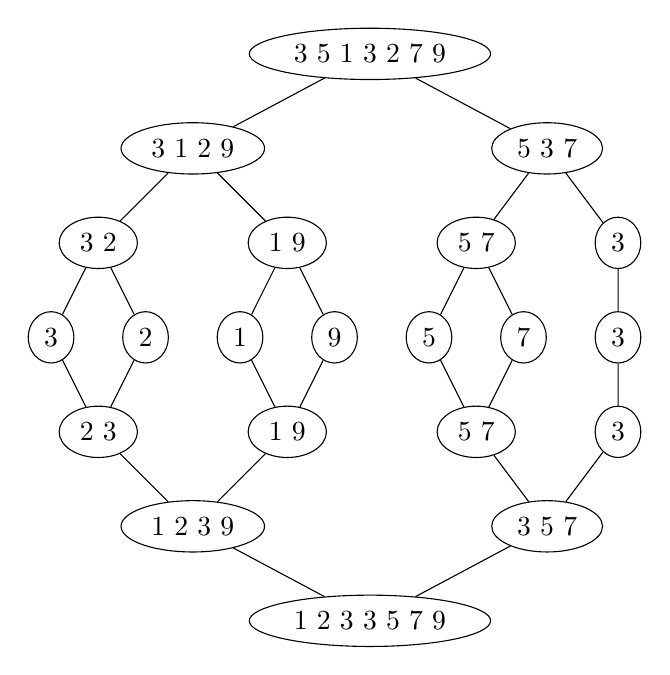
\begin{tikzpicture}[scale=1.2]
	\node [draw,ellipse] at (3.375,3) (head) {3 5 1 3 2 7 9};
	\node [draw,ellipse] at (1.5,2) (1) {3 1 2 9};
	\node [draw,ellipse] at (5.25,2) (2) {5 3 7};
	\node [draw,ellipse] at (.5,1) (3) {3 2};
	\node [draw,ellipse] at (2.5,1) (4) {1 9};
	\node [draw,ellipse] at (4.5,1) (5) {5 7};
	\node [draw,ellipse] at (6,1) (6) {3};
	\node [draw,ellipse] at (0,0) (7) {3};
	\node [draw,ellipse] at (1,0) (8) {2};
	\node [draw,ellipse] at (2,0) (9) {1};
	\node [draw,ellipse] at (3,0) (10) {9};
	\node [draw,ellipse] at (4,0) (11) {5};
	\node [draw,ellipse] at (5,0) (12) {7};
	\node [draw,ellipse] at (6,0) (13) {3};
	\node [draw,ellipse] at (.5,-1) (14) {2 3};
	\node [draw,ellipse] at (2.5,-1) (15) {1 9};
	\node [draw,ellipse] at (4.5,-1) (16) {5 7};
	\node [draw,ellipse] at (6,-1) (17) {3};
	\node [draw,ellipse] at (1.5, -2) (18) {1 2 3 9};
	\node [draw,ellipse] at (5.25, -2) (19) {3 5 7};
	\node [draw,ellipse] at (3.375,-3) (20) {1 2 3 3 5 7 9};

	\path [draw] (1) -- (head) -- (2);
	\path [draw] (3) -- (1) -- (4);
	\path [draw] (5) -- (2) -- (6);
	\path [draw] (7) -- (3) -- (8);
	\path [draw] (9) -- (4) -- (10);
	\path [draw] (11) -- (5) -- (12);
	\path [draw] (13) -- (6);
	\path [draw] (7) -- (14) -- (8);
	\path [draw] (9) -- (15) -- (10);
	\path [draw] (11) -- (16) -- (12);
	\path [draw] (13) -- (17);
	\path [draw] (14) -- (18) -- (15);
	\path [draw] (16) -- (19) -- (17);
	\path [draw] (18) -- (20) -- (19);
	\end{tikzpicture}\\*
	\newline
	Quicksort (using the first element in the list as a pivot):\\*
	\newline
	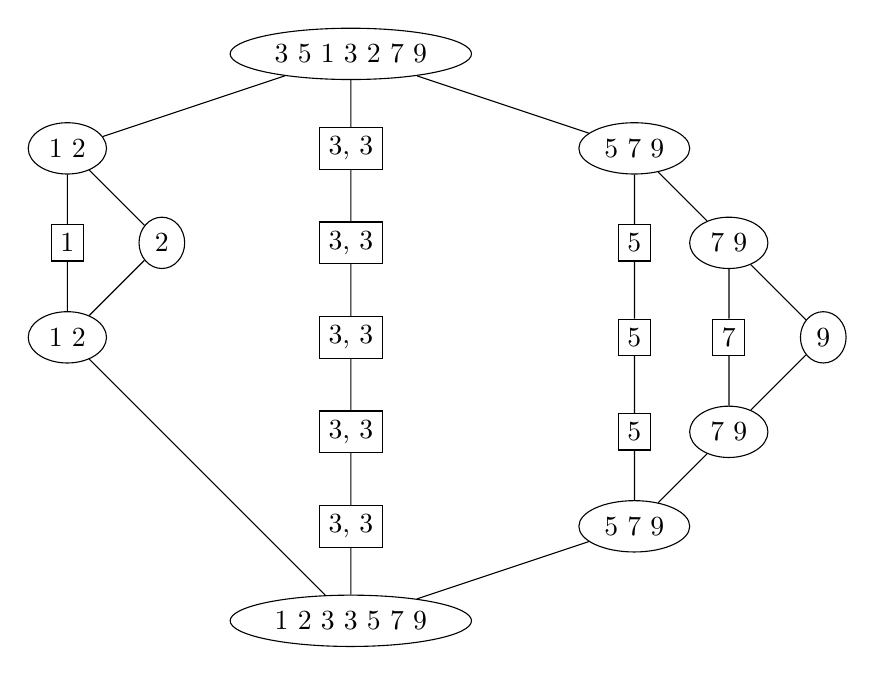
\begin{tikzpicture}[scale=1.2]
	\node [draw] at (4,0) (4) {3, 3};
	\node [draw] at (7,0) (5) {5};
	\node [draw] at (8,0) (6) {7};
	\node [draw,ellipse] at (9,0) (7) {9};
	\node [draw] at (1,1) (8) {1};
	\node [draw, ellipse] at (2,1) (9) {2};
	\node [draw] at (4,1) (10) {3, 3};
	\node [draw] at (7,1) (11) {5};
	\node [draw,ellipse] at (8,1) (12) {7 9};
	\node [draw, ellipse] at (1,2) (13) {1 2};
	\node [draw] at (4,2) (14) {3, 3};
	\node [draw,ellipse] at (7,2) (15) {5 7 9};
	\node [draw,ellipse] at (4,3) (16) {3 5 1 3 2 7 9};
	\node [draw] at (4, -1) (19) {3, 3};
	\node [draw] at (7,-1) (20) {5};
	\node [draw, ellipse] at (8,-1) (21) {7 9};
	\node [draw, ellipse] at (1,0) (22) {1 2};
	\node [draw] at (4,-2) (23) {3, 3};
	\node [draw, ellipse] at (7,-2) (24) {5 7 9};
	\node [draw, ellipse] at (4,-3) (25) {1 2 3 3 5 7 9};

	\path [draw] (8) -- (13);
	\path [draw] (8) -- (22);
	\path [draw] (9) -- (22);
	\path [draw] (9) -- (13);
	\path [draw] (4) -- (10) -- (14) -- (16);
	\path [draw] (5) -- (11) -- (15);
	\path [draw] (6) -- (12);
	\path [draw] (7) -- (12) -- (15) -- (16);
	\path [draw] (13) -- (16);

	\path [draw] (22) -- (25);
	\path [draw] (4) -- (19) -- (23) -- (25);
	\path [draw] (5) -- (20) -- (24);
	\path [draw] (6) -- (21);
	\path [draw] (7) -- (21) -- (24) -- (25);

	\end{tikzpicture}
    \end{answer}

\end{enumerate}
\end{document}
